\documentclass[12pt,space]{ctexart} %ans
\usepackage{GKExam}
\usepackage{tikz}
\usepackage{graphicx}
\usepackage{float}
\usepackage{caption}

\usetikzlibrary{positioning, shapes.geometric}
\begin{document}\zihao{5}
\juemi% 输出绝密
\biaoti{2016年普通高等学校招生全国统一考试}
\fubiaoti{上海\hspace{2em}数学试卷(理工农医类)}
{\heiti 考生注意:}
\begin{enumerate}[itemsep=-0.3em,topsep=0pt]
\item 本试卷共 \pageref{LastPage} 页,23道试题,满分为150分,考试时间为120分钟.
\item 本考试分设试卷和答题纸. 试卷包括试题与答题要求. 作答必须涂(选择题)或写(非选择题)在答题纸上,在试卷上作答一律不得分.
\item 答卷前,务必用钢笔或圆珠笔在答题纸正面清楚地填写名字、准考证号,并将核对后的条形码贴在指定位置上,在答题纸反面清楚地填写名字.
\end{enumerate}

\section{填空题(本大题共有14题,满分56分)考生应在答题纸相应编号的空格内直接填写结果,每个空格填对得4分,否则一律得零分.}
\begin{enumerate}[itemsep=-0.3em,topsep=0pt]

  \item 设$x\in R$,则不等式$|x-3|<1$的解集为\blank{$(2,4)$}.
  \item 设$\displaystyle{z=\frac{3+2i}{i}}$,其中$i$为虚数单位,则$\text{Im} z=$\blank{-3}.
  \item 已知平行直线$l_1: 2x+y-1=0$,$l_2: 2x+y+1=0$,则$l_1$,$l_2$的距离\blank{$\frac{2\sqrt{5}}{5}$}.
  \item 某次体检,6位同学的身高(单位:米)分别为1.72,1.78,1.75,1.80,1.69,1.77则这组数据的中位数是\blank{$1.77$}(米).
  \item 已知点$(3,9)$在函数$f(x)=1+a^x$的图像上,则$f(x)$的反函数$f^{-1}(x)=$\blank{$log_2(x-1)$}.
  \item 如图,在正四棱柱$ABCD-A_1B_1C_1D_1$中,底面$ABCD$的边长为3,$BD_1$与底面所成角的大小为$\displaystyle{\arctan{\frac{2}{3}}}$,
        则该正四棱柱的高等于\blank{$2\sqrt{2}$}.
  \item 方程$3\sin x=1+\cos 2x$在区间$[0,2\pi]$上的解为\blank{$30^{\circ}$或$150^{\circ}$}.
  \item 在$\displaystyle{\left (\sqrt[3]{x}-\frac{2}{x}\right )^n}$的二项式中,所有项的二项式系数之和为256,则常数项等于\blank{112}.
  \item 已知$\triangle ABC$的三边长分别为3,5,7,则该三角形的外接圆半径等于\blank{$\frac{7\sqrt{3}}{3}$}.
  \item 设$a>0$,$b>0$,若关于$x$,$y$的方程组$\begin{cases}ax+y=1\\x+by=1\end{cases}$无解,则$a+b$的取值范围是\blank{$[2,+\infty)$}.
  \item 无穷数列$\{a_n\}$由$k$个不同的数组成,$S_n$为$\{a_n\}$的前$n$项和. 若对任意$n\in N^*$,$S_n\in \{2,3\}$,则$k$的最大值为\blank{$4$}.
  \item 在平面直角坐标系中,已知$A(1,0)$,$B(0,-1)$,$P$是曲线$y=\sqrt{1-x^2}$上一个动点,
        则$\overrightarrow{BP}\cdot \overrightarrow{BA}$的取值范围是\blank{$[0,1+\sqrt{2}]$}.
  \item 设$a,b\in R$,$c\in [0,2\pi)$,若对任意实数$x$都有$\displaystyle{2\sin\left (3x-\frac{\pi}{3}\right )=a\sin(bx+c)}$,
        则满足条件的有序实数组$(a,b,c)$的组数为\blank{4}.

  \begin{minipage}[h][4em][t]{.7\textwidth}
    \item 如图,在平面直角坐标系$xOy$中,$O$为正八边形$A_1A_2\cdots A_8$的中心,$A_1(1,0)$. 任取不同的两点$A_i$,$A_j$,
    $P$ 满足 $\overrightarrow{OP} + \overrightarrow{OA_i} + \overrightarrow{OA_j} = \overrightarrow{0}$,
    则点$P$落在第一象限的概率是\blank{Unknown}.
  \end{minipage}
  \begin{minipage}[h][35pt][t]{.25\textwidth}
    \centering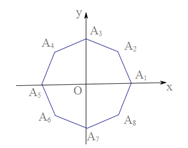
\includegraphics[width=0.8\textwidth]{Image/sh-14.png}
  \end{minipage}

\end{enumerate}

\section{选择题(本大题共有4题,满分20分)}
\begin{enumerate}[itemsep=-0.3em,topsep=0pt, resume]

  \item 设$\alpha\in R$,则“$\alpha>1$”是“$\alpha^2>1$”的
  \begin{tasks}(2)
    \task 充分非必要条件 \task 必要非充分条件 \task 充要条件 \task 既非充分也非必要条件
  \end{tasks}\vspace{1em}
  
  \begin{minipage}[h][5em][t]{.6\textwidth}
    \item 下列极坐标方程中,对应的曲线为右图的是
    \begin{tasks}(2)
      \task $\rho=6+5\cos\theta$ \task $\rho=6+5\sin\theta$ \task $\rho=6-5\cos\theta$ \task $\rho=6-5\sin\theta$
    \end{tasks}
  \end{minipage}
  \begin{minipage}[h][4em][b]{.3\textwidth}
    \centering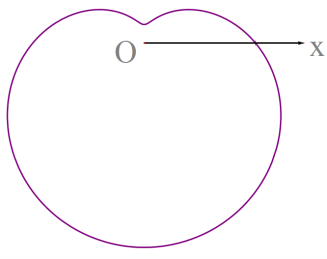
\includegraphics[width=0.45\textwidth]{Image/sh-16.png}
  \end{minipage}

  \item 已知无穷等比数列$\{a_n\}$的公比为$q$,前$n$项和为$S_n$,且$\lim_{n\rightarrow\infty}S_n=S$. 下列条件中,
        使得$2S_n<S\,(n\in N^*)$恒成立的是
  \begin{tasks}(2)
    \task $a_1>0$,$0.6<q<0.7$ \task $a_1<0$,$-0.7<q<-0.6$ 
    \task $a_1>0$,$0.7<q<0.8$ \task $a_1<0$,$-0.8<q<-0.7$ 
  \end{tasks}

\end{enumerate}

%%%%%%%%%%%%%%%%%%%%%%%%%%%%%%%%%%%%%%%%%%%%%%%%%%%%%%%%%%%%%%%%%%%%%%%%%%
%---------------------------------结束------------------------------------
%%%%%%%%%%%%%%%%%%%%%%%%%%%%%%%%%%%%%%%%%%%%%%%%%%%%%%%%%%%%%%%%%%%%%%%%%%
\clearpage

\end{document}
